\documentclass[a4paper]{article}
\usepackage[margin=1in]{geometry}
  \usepackage{times}
  \usepackage{helvet}
  \usepackage{courier}
  \usepackage{graphicx}
  \usepackage[T1]{fontenc}
  \usepackage[utf8]{inputenc}
  \frenchspacing
  \setlength{\pdfpagewidth}{21.0cm}
  \setlength{\pdfpageheight}{29.7cm}
  \pdfinfo{
  /Title (Crazy, stupid, love.)
  /Author (Victor Chibotaru, Larissa Laich, Galina Peycheva, Ondrej Skopek)}
  \setcounter{secnumdepth}{0}
  \newcommand{\TODO}[1]{\begin{center}\large\textbf{TODO:} #1\end{center}}
\begin{document}

\title{Crazy, stupid, love.}
\author{Victor Chibotaru\quad Larissa Laich\quad Galina Peycheva\quad Ondrej Skopek\\
  Team 5\\
  Department of Computer Science\\
  ETH Zurich\\
  Switzerland\\
  \texttt{\{viktorc, llaich, galinap, oskopek\}@ethz.ch}
}
\maketitle
\begin{abstract}
  \begin{quote}
    You attempt to penetrate a company's internal employee registry and
    regain the girl's phone number. To do this, you have to overcome
    multiple layers of security. You want to get SSH access to the company's
    server. To do that, you need to get user credentials using a
    server-side XXE vulnerability.
    To obtain the first part of the admin's SSH password, you
    exploit an server-side template injection vulnerability in the
    admin's contact form, and obtain their 2FA token by
    reverse engineering a custom-made 2FA app.
    Using those secrets, you log in to the admin's server
    and get an encrypted ZIP file of the company's internal employee
    registry. Using a Known Plaintext ZIP vulnerability, you
    decrypt and decompress the file, and get the phone number you lost!
  \end{quote}
\end{abstract}

\TODO{Add references where appropriate!}
\TODO{Enhance mitigation part?}

\section{Backstory}

One day at PapperlaPub, you meet this amazing girl and start a long
conversation with her. You are super excited: Despite your computer
science background, you managed to get her phone number! The next
morning, when you sober up, you start thinking about your amazing
evening, and want to text her. Where did you put her phone number? After
desperately searching for hours, you realize that you've
probably lost it on your way home! What should you do now?

Fortunately, you remember that she works at Gügli. So you try to call
the company but the secretary tells you that she will not provide any
data about employees, and also will not forward any message to the girl.
You are very upset. How can anybody be that mean? Suddenly, it hits you.
The girl was complaining about their local sysadmin a lot. Should you
try to get the phone number by hacking into the Gügli system? It's a
long shot, but it's definitely worth a try!

\section{Requirements}

\noindent We will need two VMs:

\begin{enumerate}
  \item Client VM
  \item Server VM (Linux, any version/distro)
        \begin{enumerate}
          \item Web server (custom)
          \item SSH daemon
          \item Python
        \end{enumerate}
\end{enumerate}

\noindent Client tools:

\begin{itemize}
  \item pkcrack
  \item Python
  \item Java, JDGUI
  \item SSH client + sshpass
  \item Internet access
  \item nmap
\end{itemize}

\section{Learning goal}

In practice, getting root access is a multi-step process. Systems and
networks are protected on multiple levels. (Un)fortunately, each of the
steps often has several vulnerabilities. In our challenge, step:

\begin{enumerate}
  \item teaches you that
        \begin{enumerate}
          \item \TODO{XXE learning goal}
          \item not sanitizing user input is a bad idea every time;
        \end{enumerate}

  \item teaches you that
        \begin{enumerate}
          \item \TODO{SSTI learning goal}
          \item not sanitizing user input is a bad idea every time;
        \end{enumerate}

  \item teaches you that
        \begin{enumerate}
          \item even inside a secured system, protecting yourself and all other systems
                is still important,
          \item two factor authentication is important, but also important to get right,
          \item not sanitizing user input is a bad idea every time;
        \end{enumerate}

  \item teaches you that
        \begin{enumerate}
          \item sysadmins might not be the security gurus they pretend to be,
          \item storing your company's important details locally in an encrypted zip
                file is a very bad idea, even if only the admin has access.
        \end{enumerate}

\end{enumerate}

\section{Mission}

Gain access to the company's employee registry data containing the
girl's lost number! Steps:

\begin{enumerate}
  \item Get a user's credentials by exploiting the certificate web query form.
  \item Get the admin's password (they check the forum quite often).
  \item Get access to the admin's 2FA token.
  \item Get the encrypted ZIP file of employee records and decrypt it.
\end{enumerate}

\section{Mitigation}

\begin{enumerate}
  \item Thoroughly check user input!
      Do not leave debugging info lying around. Lock down the permissions
      of users that are running systems/web apps.
  \item Once again, thoroughly check user input! Do not attempt to
      ``interpret'' it --- escape it properly. Never write down important passwords,
        at least in a way that is accessible online in any way.
  \item Do not create your own and buggy software for two factor authentication. Use
        trusted, proven, and updated versions of software. Do input
        validation!
  \item Never store important information on servers accessible from the
        external network. Do not store them in encrypted ZIP files. Also,
        store unrelated data separately.
\end{enumerate}

\section{Type of challenge}

This is an online challenge.

\section{Category}

\begin{itemize}
  \item Penetration Testing
  \item Web Security
  \item Reverse Engineering
  \item Cryptography
\end{itemize}

\section{Hints}

\begin{enumerate}
    \item \texttt{/hints}
\end{enumerate}

\section{Step-by-step instructions}

For an overview, see Figure \ref{fig:diag}.

\TODO{Clarify the steps and instructions.}
\TODO{Screenshots}

\begin{enumerate}
  \item Do network reconnaissance.
  \item Find the server VM, enumerate all the open ports using nmap, figure
        out which services are running for each of the ports.
  \item Get user access to the company's server.
        \begin{enumerate}
          \item Exploit one of the server's functions.
              Use XXE to attack the service for listing the users and their public keys.
                The service will accept ``smart'' queries written in XML to filter out
                the search results, but luckily for you, the parser will be
                vulnerable to XXE. Thus, it is possible to extract files
                from the server.
          \item Using the XXE exploit you can dump a list of
                forum users and their password hashes, forgotten in a comment
                in the actual web app source files.
          \item Recover the passwords using a rainbow table.
        \end{enumerate}

  \item Steal the admin's password.
        \begin{enumerate}
          \item The company's admin contact form is vulnerable to reflected XSS. The attacker is
              hence able to post an XSS message to the Q\&A system. Then the admin, who
                checks it periodically, will run into this code and his browser
                will execute it. However, the admin is not accesing the system using a browser!
          \item The webapp uses the jinja templating engine. Run a server-side template
              injection attack and extract the previously unobtainable \texttt{view.py} file.
              Find the admin's SSH password.
        \end{enumerate}

  \item Reverse engineer the APK downloaded from the web app.
        \begin{enumerate}
          \item Find the 2FA app in the menu and download it.
          \item Use a java decompiler and check out the algorithm.
              Notice that it returns only the last three decimal digits!
          \item Brute-force the obtained password appended with a 2FA token
              using \texttt{ssh} and \texttt{sshpass}.
              You have gained access to the admin's account using SSH!
        \end{enumerate}

  \item Find the \texttt{~/database\_backup/backup.zip}. Read through the \texttt{contents.txt} file next to it:
          it describes the contents of the ZIP archive. Based on the fact that the ZIP archive
          also contains the secret \texttt{db.txt} file, you can use a Known Plaintext
        Attack (download PkCrack). Run:
        \begin{quote}
            \texttt{pkcrack -p contents.txt -e contents.txt -P contents.zip \textbackslash}\\
            \texttt{-C backup.zip -d output.zip}\\
        \end{quote}
        \TODO{Remove the ca cert from the zip?}
        \TODO{Remove all the hints/comments about CA certs and the cert login}.

  \item Find the girl's number in the DB!

\end{enumerate}

\begin{figure}
    \begin{center}
    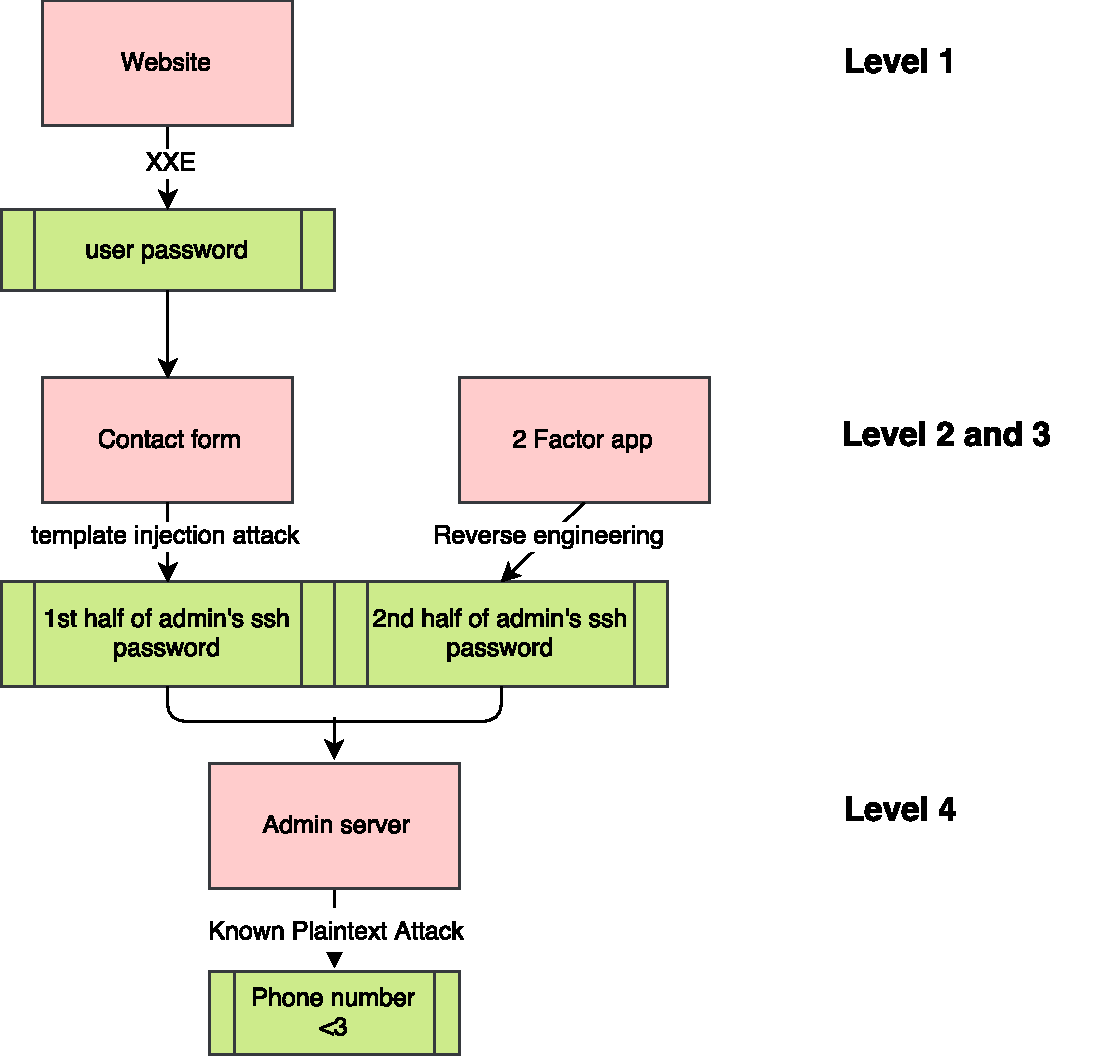
\includegraphics[width=0.7\textwidth]{images/diagram}
    \end{center}
    \caption{An overview of our challenge. The system's vulnerabilities
    are displayed as red boxes and obtained data in green boxes. The attacks
    to exploit the vulnerabilities are written on the edges.}
    \label{fig:diag}
\end{figure}


\section{Implementation}

\TODO{Add implementation details --- describe the system implementation, what challenges there were, \ldots}
\TODO{Add references for attacks!}

\subsection{Setup}

\begin{enumerate}
    \item Import the two VMs into VirtualBox.
    \item Start the server VM (headless).
    \item Login to the client VM using \texttt{hacker/compass}.
    \item The server is accessible at the dns name \texttt{gugli} \TODO{hosts file entry client-side + static IPs in a subnet}.
\end{enumerate}

\end{document}